\documentclass[11pt,a4paper]{scrartcl}
\usepackage[czech]{babel}
\usepackage[utf8]{inputenc}
\usepackage{graphicx}
\usepackage{float}
\graphicspath{{./img/}}

\begin{document}
	\begin{figure}[h!]
		\centering
		
\includegraphics[bb= 0 0 820 445 , width=75mm]{favlogo.jpg}
	\end{figure}
	
	\vspace{5cm}
	
	{\centering
		{\huge KIV/OS - Semestrální práce}\\[1em]
		{\large Simulátor operačního systému}\\[7,5cm]
	}
	
	\begin{center}
		\begin{tabular}{l r}
		student: & Daniel HRYZBIL, Anežka JÁCHYMOVÁ, Zdeněk VALEŠ\\
		datum: & 29.11.2019\\
		\end{tabular}
	\end{center}
	
	\thispagestyle{empty}
	\newpage
	
	\section{Zadání}
	\begin{enumerate}
		\item 	Vytvořte virtuální stroj, který bude simulovat OS
		\item 	Součástí bude shell s gramatikou cmd, tj. včetně exit
		\item 	Vytvoříte ekvivalenty standardních příkazů a programů:
		\begin{enumerate}
			\item echo, cd, dir, md, rd, type, find /v /c"" (tj. co dělá wc v unix-like prostředí), sort, tasklist, shutdown
			
			\begin{enumerate}
				\item	cd musí umět relativní cesty
				\item	echo musí umět @echo on a off
				\item	type musí umět vypsat jak stdin, tak musí umět vypsat soubor
			\end{enumerate}
		
			\item	Dále vytvoříte programy rgen a freq
			\item	rgen bude vypisovat náhodně vygenerovaná čísla v plovoucí čárce na stdout, dokud mu nepřijde znak Ctrl+Z //EOF
			\item	freq bude číst z stdin a sestaví frekvenční tabulku bytů, kterou pak vypíše pro všechny byty s frekvencí větší než 0 ve formátu: “0x\%hhx : \%d”
		\end{enumerate}
		\item 	Implementujte roury a přesměrování
		\item 	Nebudete přistupovat na souborový systém, ale použijete simulovaný disk
		
		\begin{enumerate}
			\item 	Za 5 bonusových bodů můžete k realizaci souborového systému použít semestrální práci z KIV/ZOS - tj. implementace FAT.
		\end{enumerate}
	\end{enumerate}

	\section{Kernel}
	
	\subsection{Procesy a vlákna}
	
	\subsection{Filesystem}
	
	\begin{figure}
		\centering
		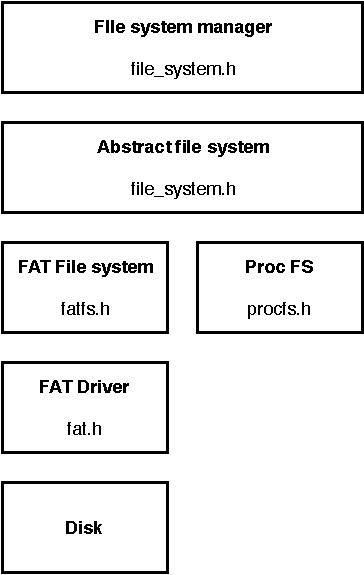
\includegraphics[height=9cm]{fs-layers.pdf}
		\caption{Struktura správy souborového systému}
		\label{fig:fs-layers}
	\end{figure}

	\begin{figure}
		\centering
		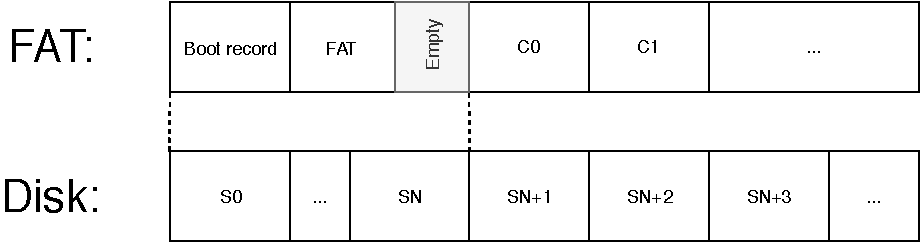
\includegraphics[width=12cm]{fat-rozdeleni-disku.pdf}
		\caption{Uložení FAT souborového systému na disk}
		\label{fig:fat-disk-struct}
	\end{figure}
	
	\subsection{Pipe}
	
	\section{RTL}
	
	\section{Shell a uživatelské příkazy}
	
	\section{Závěr}
	
\end{document}
